\chapter{Solutions}

Maintenant que la problématique a été établie, le but était de définir les caractéristiques clés de notre problème.


\section{Caractéristiques du problème}
Notre agent assistant devra implémenter un système de dialogue avec l'utilisateur répondant aux critères suivants :
\begin{itemize}
	\item le dialogue doit permettre de réunir un ensemble d'informations (heure, jour);
 	\item l'ordre des informations recueillies n'est pas défini (on peut donner l'heure avant le jour, ou le contraire);
 	\item l'entrée de l'utilisateur est textuelle ou bien vocale et en langage naturel ;
 	\item la réponse fournie par l'agent est elle aussi textuelle ou vocale ;
 	\item la mise en place est rapide, réalisable dans un projet de type \textit{Proof of Concept}.
\end{itemize}

\section{Solutions scientifiques}

\subsection{Gestion de dialogue}
Notre problématique générale est donc d'implémenter un système de dialogue. Plusieurs solutions existent pour ce genre de problème et nous avons donc étudié les plus répandues pour choisir celle (ou celles) qui serait la plus adéquate à notre problème. Notamment avant de pouvoir réaliser la conception, il nous a fallu définir quelle serait notre gestion de dialogue (par formulaire, état de l'information, etc.). Ce choix était primordial car il risquait fortement d'impacter la manière dont nous allions réaliser notre projet et par conséquent notre conception.


\FloatBarrier

\subsubsection{Le dialogue par état de l'information ou ISU (Information State Update)}

L'approche ISU (Information State Update) est un cadre de gestion de dialogue. Le principe des différentes théories ISU est l'idée d'un état de l'information qui est modifié par des règles de mise à jour déclenchées par des mouvements de dialogue. En résumé, une théorie de dialogue ISU consiste en :
\begin{itemize}
	\item une caractérisation des états de l'information, qui décrit tous les aspects du contexte du dialogue ainsi que les facteurs de motivation internes ;
	\item un ensemble de mouvements de dialogue. Ceux-ci sont généralement associés à des énoncés ou à des parties d'énoncés par les entités participants au dialogue ;
	\item un ensemble de règles de mise à jour, qui régissent la mise à jour de l'état des informations. Une règle de mise à jour consiste en une liste de conditions préalables sur l'état d'information et une liste d'effets qui modifient l'état d'information ;
	\item une stratégie de mise à jour pour décider quelle(s) règle(s) sélectionner à un moment donné.
\end{itemize}

~\\\indent
Une librairie Python permet de faciliter l'implémentation de ce paradigme de gestion de dialogue : \texttt{Trindikit}. 

~\\\indent
Cette solution pourrait s'adapter à notre projet car elle est très générale et peut se prêter à un grand éventail de dialogues possibles. Mais elle est aussi très complexe et nécessite une étude approfondie des théories ISU ainsi qu'une formation complète sur la librairie \texttt{Trindikit} qui est par ailleurs peu documentée et peu mise à jour. 

~\\\indent
Cette solution ne satisfait donc pas le critère : \og la mise en place doit être rapide, réalisable dans un projet de type \textit{Proof of Concept} \fg. 

Nous avons donc décidé d'écarter cette solution.

\FloatBarrier

\subsubsection{Le dialogue à structure hiérarchique}
La dialogue à structure hiérarchique est une méthode de gestion de dialogue qui se base sur une ou plusieurs tâches précises. Elle comprend une architecture deux tiers (figure \ref{architecture-hierarchique}). Une partie qui s'occupe des aspects spécifiques du dialogue en fonction de la tâche voulue. Et une autre partie qui s'occupe du contrôle et du flux de dialogue indépendamment des spécificités de ce dernier. 

Le principe est le suivant: \\
la partie spécifique aux tâches est composée d'arbres chacun dédié à une tâche ou sous-tâche (figure \ref{architecture-hierarchique}). 

Il y a quatre type d'agents :
\begin{itemize}
	\item Informer : envoie une information à l'utilisateur ;
	\item Demander : demande une information à l'utilisateur ;
	\item Attendre : attend une information de l'utilisateur sans lui demander ;
	\item Exécuter : exécute une action (accès à une base de données, appel à un API, etc.). 
\end{itemize} 

~\\\indent
Les agents composant cet arbre seront alors placés dans une pile d'exécution qui sera changeante à chaque étape du dialogue en fonction de l'arbre de départ et des dépendances entre chaque tâche (figure \ref{execution-hierarchique}). 

\textit{Exemple: il est nécessaire de s'identifier avant d'accéder à ses e-mails}. Et cette pile sera exécutée dans l'ordre.

~\\\indent
La partie indépendante des spécificités des tâches du dialogue est composée de cette pile d'agent, ainsi que d'un agenda des attentes (\textit{expectation agenda}), qui résume toutes les informations que l'agent attend à chaque phase du dialogue. Cet agenda permet notamment de gérer la sur-information que l'utilisateur peut donner. 

\textit{Exemple: On demande à l'utilisateur quel jour il veut programmer son réveil et il répond \og Demain à 8h \fg, 8h est alors considéré comme de la sur-information mais l'agenda permet de la traiter pour ne pas à avoir à demander l'heure à la phase suivante}.


\FloatBarrier
 
 
 
\begin{figure}[!h]
	%https://fr.slideshare.net/cybrshin/commerce-chatbot-dialog-manager
	\centering
	\begin{minipage}{.45\textwidth}
		\centering
		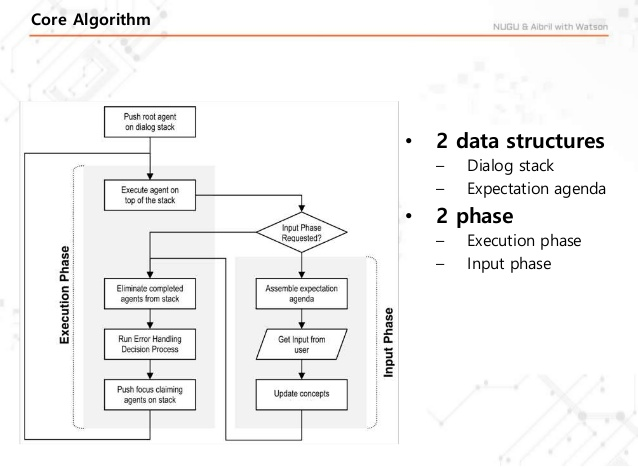
\includegraphics[width=1\textwidth]{images/hierarchique_manager.jpg}
		\caption{Principe d'exécution d'un dialogue à structure hiérarchique}
		\label{execution-hierarchique}
	\end{minipage}%
	\begin{minipage}{0.45\textwidth}
		\centering
		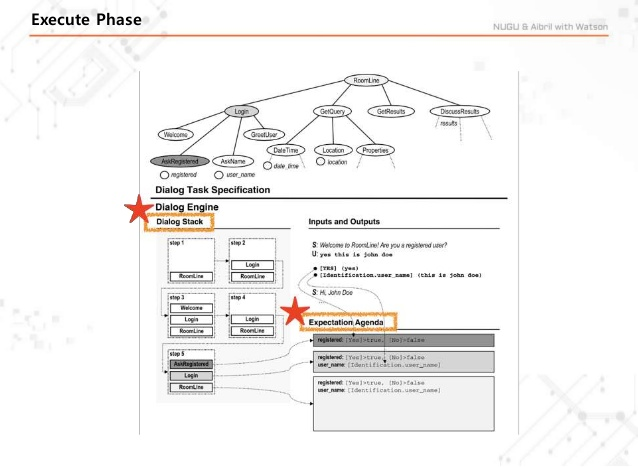
\includegraphics[width=1\linewidth]{images/hierarchique_manager_2.jpg}
		\caption{Architecture d'un dialogue à structure hiérarchique}
		\label{architecture-hierarchique}
	\end{minipage}
\end{figure}

\FloatBarrier

Cette solution pourrait parfaitement s'adapter à notre projet car elle permet d'implémenter un dialogue ayant un but spécifique et peut aussi s'incrémenter facilement en cas d'amélioration possible de notre agent. 

Elle peut aussi permettre de récolter des informations dans n'importe quel ordre. 

En revanche la seule implémentation connue et répandue de cette technique est \textit{Ravenclaw} qui est un framework en \texttt{C++} et qui ne tourne que dans un environnement Windows. Ne maitrisant pas tous ce langage ou cet environnement, nous avons décidé d'abandonner cette solution. 

\subsubsection{Le dialogue par formulaire}
Le dialogue par formulaire est une technique de gestion de dialogue qui permet à l'agent assistant de récolter des informations \emph{via} un dialogue avec l'utilisateur (pour notre projet : alarme, heure et jour). 

L'agent pourra enregistrer dans différents champs de son formulaire les informations récoltées. Il pourra ensuite envoyer les données du formulaire à un module de traitement qui effectuera des actions en conséquence de ces données. Le dialogue peut être initié par les deux parties : soit l'agent, soit l'utilisateur. L'agent cherchera à récolter les informations pour remplir le formulaire. Les informations peuvent être récoltées dans n'importe quel ordre et en un seul ou plusieurs échange(s) de messages.

La figure \ref{form-dialog} illustre ce principe.
\begin{figure}[H]
\centering
    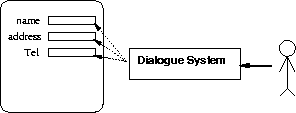
\includegraphics[scale=0.7]{images/slot.png} %www.dfki.de
    \caption{Principe du dialogue par formulaire}
    \label{form-dialog}
\end{figure}

Cette solution serait très avantageuse pour notre projet. 
En effet, elle répond à tous les critères énoncés précédemment : 
\begin{itemize}
    \item elle permet de réunir des informations (ici dans un formulaire) ;
    \item l'ordre des informations n'est pas défini ;
    \item l'entrée de l'utilisateur est en langage naturel ainsi que la réponse de l'agent ;
    \item la mise en place peut sembler être assez longue mais une application en ligne, \texttt{DialogFlow}, permet de faciliter ceci et de rendre l'implémentation d'un dialogue par formulaire plus rapide.
\end{itemize}
\FloatBarrier


\FloatBarrier
\subsection{Analyse syntaxique}
En plus de la gestion de dialogue, un système de dialogue a besoin d'un analyseur syntaxique, c'est pourquoi il est intéressant d'étudier le sujet. 

Le principe d'un analyseur syntaxique est de mettre en évidence la structure du texte envoyé par l'utilisateur. Ainsi l'analyseur peut savoir quel est le verbe de la phrase, les compléments d'objets, le sujet etc... 

Il retourne alors un arbre syntaxique (figures \ref{arbre-syntaxique} et \ref{arbre-syntaxique2}). 

~\\\indent Par exemple pour notre projet, si dans l'arbre syntaxique le verbe est \og \textit{mettre} \fg{} et que le complément d'objet est \og \textit{réveil} \fg, l'agent \og comprend \fg{} qu'il doit programmer un réveil. Il va donc continuer le dialogue dans ce sens en demandant l'heure et le jour où le réveil doit être programmé si ces informations lui manquent.

\begin{figure}[!h]
	\centering
	\begin{minipage}{.5\textwidth}
		\centering
		%www.linguistes.com
		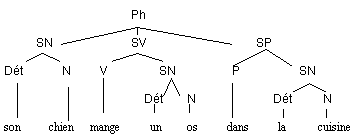
\includegraphics[width=0.9\textwidth]{images/arbre.png}
		\caption{Exemple d'arbre syntaxique}
		\label{arbre-syntaxique}
	\end{minipage}%
	\begin{minipage}{0.5\textwidth}
		\centering
		%http://french.chass.utoronto.ca/
		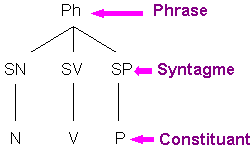
\includegraphics[width=0.9\linewidth]{images/arbre2.png}
		\caption{Hiérarchie de l'arbre syntaxique}
		\label{arbre-syntaxique2}
	\end{minipage}
\end{figure}

~\\\indent
Cette partie des systèmes de dialogues est intéressante mais nous n'avons pas approfondi nos recherches à ce sujet. En effet comme nous l'expliquerons dans la prochaine partie, nous avons choisi une solution pour la gestion de dialogue qui a son propre analyseur syntaxique et sémantique.

\subsection{Description de la solution retenue}
Après cette analyse des différentes solutions existantes, nous avons décidé d'implémenter la solution de dialogue par formulaire (pour les raisons évoquées précédemment). 

Plus précisément nous avons choisi d'utiliser \texttt{DialogFlow}. 

C'est une plateforme qui permet de rapidement implémenter un système de dialogue par formulaire. Elle effectue une analyse syntaxique et sémantique grâce à des solutions de \textit{Machine Learning} et de \emph{Text Mining}. 

L'analyse sémantique permet, entre autre, de pouvoir \emph{tagger} des entités (date, lieu, nom). Ces \emph{tags} permettront le remplissage du formulaire.